\section{Mediciones}

Se realizaron mediciones en base a crear sets de distinta cantidad de
elementos, con la cantidad de subsets y la cantidad de elementos por subset
siendo proporcional a la cantidad de elementos.

Para asegurar la validez de las comparaciones todas las mediciones fueron
realizadas sobre los mismos sets de datos para los m\'etodos que est\'an siendo
comparados. Los elementos fueron generados por los valores pseudoaleatorios del
lenguaje (el m\'odulo \texttt{random}) con la misma \textit{seed}.

\subsection{Backtracking vs. Programación Lineal}

\begin{figure}[H]
    \centering
    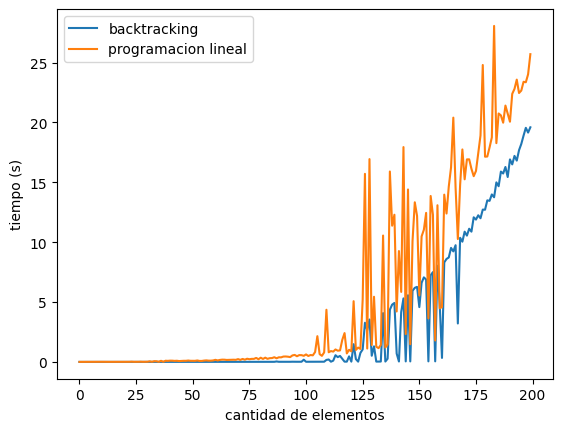
\includegraphics[width=1\textwidth]{img/backvslp.png}
\end{figure}

Backtracking obtiene mejores tiempo de ejecución que programación lineal para
encontrar la solución óptima.

\subsection{Algoritmos de aproximaci\'on}

\begin{figure}[H]
    \centering
    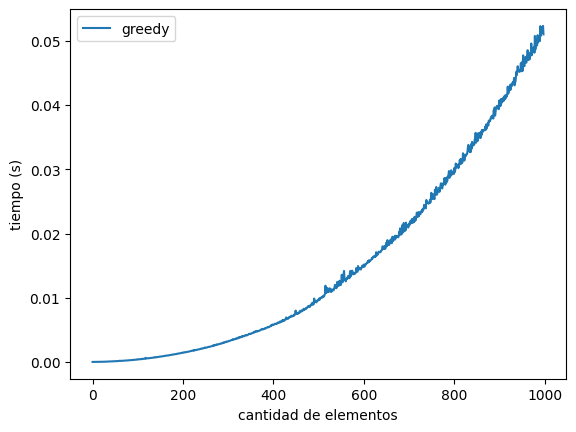
\includegraphics[width=0.49\textwidth]{img/greedy.png}
    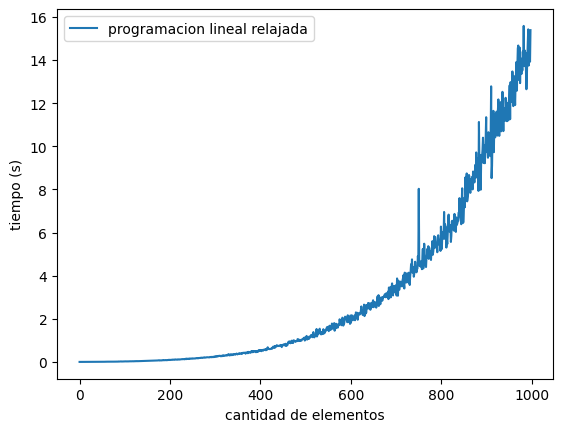
\includegraphics[width=0.49\textwidth]{img/pl_rlx.png}
\end{figure}

Notar la diferencia de tiempos (eje y) entre greedy y programación lineal.

\subsection{Cota de la relajaci\'on lineal}

Se realizaron mediciones para verificar la cota calculada empiricamente con un
valor de $r(A) = 20$:

\begin{figure}[H]
    \centering
    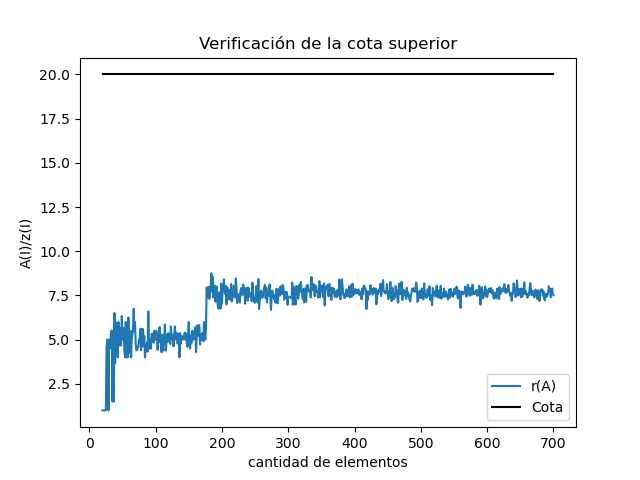
\includegraphics[width=0.8\textwidth]{img/cota.png}
\end{figure}

Vemos que $\frac{A(I)}{z(I)}$ se mantiene por debajo de la cota calculada. Cabe
aclarar que a partir de los 175 elementos se utiliz\'o una cota inferior para
$z(I)$, por lo que se ve un pico en el gr\'afico a partir de ah\'i, esta cota
inferior fue calculada por el mismo algoritmo de programaci\'on lineal relajada
porque los volumenes de datos eran inmanejables para el algoritmo exacto.
